%%%%%%%%%%%%%%%%%%%% author.tex %%%%%%%%%%%%%%%%%%%%%%%%%%%%%%%%%%%
%
% sample root file for your "contribution" to a proceedings volume
%
% Use this file as a template for your own input.
%
%%%%%%%%%%%%%%%% Springer %%%%%%%%%%%%%%%%%%%%%%%%%%%%%%%%%%


\documentclass{svproc}
\usepackage{marvosym}
%
% RECOMMENDED %%%%%%%%%%%%%%%%%%%%%%%%%%%%%%%%%%%%%%%%%%%%%%%%%%%
%
\usepackage{graphicx}
\usepackage{float}
\usepackage[boxed,vlined,ruled]{algorithm2e}

% to typeset URLs, URIs, and DOIs
\usepackage{url}
\usepackage{hyperref}
\def\UrlFont{\rmfamily}
\providecommand{\doi}[1]{doi:\discretionary{}{}{}#1}

\def\orcidID#1{\unskip$^{[#1]}$}
\def\letter{$^{\textrm{(\Letter)}}$}

%%%%%% DEBUG section %%%%%%
\newcommand*{\DEBUG}{}

\ifdefined\DEBUG
\usepackage[T2A]{fontenc}
\usepackage[utf8]{inputenc}
%\usepackage[russian]{babel}
\usepackage[usenames]{color}
%\usepackage{colortbl}
\newcommand{\FIXME}[1]{ % описание
	\colorbox{yellow}{#1}
}
\else
\newcommand{\FIXME}[1]{ % описание
}
\fi


\begin{document}
\mainmatter              % start of a contribution
%
\title{Topological approach to finding blackholes in directed networks}
%
\titlerunning{Topological black holes mining}  % abbreviated title (for running head)
%                                     also used for the TOC unless
%                                     \toctitle is used
%
\author{Denis Ivanov\inst{1} \and Alexander Semenov\inst{2}}
%
\authorrunning{Ivanov, Semenov} % abbreviated author list (for running head)
%
%%%% list of authors for the TOC (use if author list has to be modified)
\tocauthor{Denis Ivanov and Alexander Semenov}
%
\institute{Lomonosov Moscow State University, Moscow, Russian Federation \\
\email{mr.salixnew@gmail.com}
\and
JSC NICEVT, Moscow, Russian Federation\\
\email{semenov@nicevt.ru}
}

\maketitle              % typeset the title of the contribution

\begin{abstract}
In this paper we consider the problem of finding so called Blackhole pattern in directed unweighted graphs.
Firstly, we analyse already existing algorithms and approaches. Secondly, we describe how structure of a graph
affects their efficiency. Then we introduce our approach to graph preprocessing. Finally, we describe topological sort based heuristic
and provide results of experimental comparison between our approach and previously developed algorithm.
\keywords{Directed networks $\cdot$ Subgraph mining}
\end{abstract}

\section{Blackhole Search in Directed Graph}
The task of pattern mining in directed graphs finds its aplications in different areas. In 2010 Li et al.\cite{li2010mining} state
that governments are interested in detecting cases of financial fraud. They formulate the task for finding cases of illegal collaboration, and introduce dual patterns:
blackhole and volcano. Those appear when a group of traders perform operations only between each other in order to manipulate market.
Continuing study of different financial fraud casese, in 2017 Semenov et al. \cite{semenov2017survey} provided a survey of common approaches to anti - money laundering by graph mining.
There are other applications. For example, the online detection of black holes/volcanos can timely 
reflect anomalous events, such as disasters, catastrophic accidents, and therefore help keep public safety \cite{hong2015detecting}.

\subsection{Problem Statement and Preliminaries}
In this section we provide some basic notations and definitions, which will be used in this paper. In this paper we consider simplified problem formulation, applied to directed unweighted graph.

First, consider a directed graph $G = G(V,E)$, where $V$ is a set of all nodes and $E$ is a set if all edges of the graph. 
\FIXME{Мне кажется, это лишнее предложение, так не пишут в статьях:} Assume that we deal with the general case of graph, without any special restrictions, unless the opposite is stated. 

\begin{definition}
Subset of nodes $B \in V$ is called a blackhole if  the following two conditions are satisfied: 
1) Subgraph $G'(B, E')$ induced by $B$ is weakly connected, 
%$|B| \geq 2$,
and
2) there is no such pair of nodes $(u,v)$ that $u \in B$, $v \in V \backslash B$ and $(u,v) \in E$.
\end{definition}

The goal is to find in unweighted directed graph as many blackholes as possible in restricted time.

To support further discussion, we provide several more definitions.

\FIXME{Удалил возможные кратные ребра в определении 2, это важно?}
\begin{definition}
For a given directed graph $G(V,E)$ we say that sequence $v_0v_1v_2...v_{k}$ of $v_i \in V, 0 \leq i \leq k$ forms a directed path from $v_0$ to $v_k$, if there are edges $(v_{i-1}, v_i) \in E, 1 \leq i \leq k$ and $v_i \neq v_j$ for all $0 \leq i, j \leq k, i \neq j$. The length of this directed path is $k$.
\end{definition}

\begin{definition}
For a given directed graph $G(V,E)$ we say that $v \in V$ is reachable from $u \in V$ if there is a directed path that starts from $u$ and ends at $v$.
\end{definition}

\begin{definition}
For a given directed graph $G(V,E)$ if $v \in V$ is reachable from $u \in V$, then we say $u$ is a predecessor of $v$ and $v$ is a successor if $u$.
If there is an edge from $u$ to $v$, then $u$ is a direct predecessor of $v$, and $v$ is a direct successor if $u$.
\end{definition}

\begin{definition}
Set of nodes in a directed graph $G$ is called a Strongly Connected Component (SCC) if every node of $G$ is reachable from every other node of $G$.
\end{definition}

\begin{definition}
For a given directed graph $G(V,E)$. The closure of $v \in V$ is $Closure(v) = \{u\ |\ there\ is\ a\ directed\ path\ from\ v\ to\ u\} \cup \{v\}$.
In other words, a closure of node $v$ is a set of all nodes reachable from $v$, including $v$.
\end{definition}

The following lemmas are proved in \cite{li2010detecting}.

\begin{lemma}
If a node $v \in B$, where $B \subseteq V$ is a blackhole, then all the successors of $v$ are in $B$.
\end{lemma}

\begin{lemma}
If a node $v \in B$, where $B \subseteq V$ is a blackhole, then the closure of $v$ is a subset of $B$.
\end{lemma}

\begin{lemma}
Closure of $v$ forms a blackhole.
\end{lemma}

We will need the following statement to discuss issues of known approaches.
\begin{lemma}
For a given graph $G(V,E)$, SCC $S \subseteq V,\ blackhole\ B \subseteq V$ if $\ \exists v \in S: v \in B$,  then $\forall s \in S$ will be true $s \in B$.
In other words, if any node in SCC belongs to a blackhole, then all the nodes of this SCC belong to the same blackhole.
\end{lemma}
\begin{proof}
    In SCC any node is reachable from any other node. This means, that any node $v$ in SCC contains the whole SCC in its closure. By Lemma 3 the whole SCC belongs to the same blackhole as $v$. 
\end{proof}

\subsection{Related Work}

% Previously 
%Authors from the University of New Jersey gave \cite{li2010detecting} general and simplified problem formulation for blackhole search
in directed graph.

The main contributor to the blackhole detecting problem is the authors from the University of New Jersey. They both formulated the task and provided an algorithm for blackhole detection in case of unweighted directed graph \cite{li2010detecting}. 
Two years later they published an algorithm for approximate blackhole search in general case (weighted graph) \cite{li2012mining,li2014mining}. 
Hong et al \cite{hong2015detecting} had
an unusual application for blackhole mining in the city environment. They introduced an original algorithm.  

\subsection{Known issues}
In this section we shortly discuss applicability of the iBlackhole algorithm, proposed in \cite{li2010detecting}.
The iBlackhole algorithm (see Algorithm \ref{alg:iblackhole}) is designed for searching blackholes of fixed size. Potentially it has a great resource of parallelism, however this work does not cover the case of large scale graphs, as they only run their algorithm on 1500 node networks, which are quite
a small size.
Also, there are graphs, which has a small number of blackholes in relation to number of nodes. They consist
of several large SCCs and relatively small number of independent leaves (or roots). Here arise some questions considering applicability of
iBlackhole algorithm:
\begin{itemize}
\item How do we know if there are blackholes of certain size? We have to check all the possible sizes, which can take too much time even in parallel.
\item How do we reduce the search space for the brute-force stage and avoid repeatedly checking the same combinations for different candidate sizes?
\end{itemize}

Let's consider the following example:

Graph consisting of $(10^6)$ nodes, all of them form a single SCC. It means that there is only one blackhole -- the whole graph.
Unless we do not know anything about the graph structrure and do not have large enough cluster, we have one to a million chance
to efficiently choose target size of blackhole. In general case, we have to check $10^6$ possible sizes.

Another example is well-known small-world graphs \cite{watts1999networks}. It has most of its nodes in one large SCC, couple of leaves and couple of roots.
We claim that with looking from small to large size candidates in the iBlackhole algorithm we will quickly discover all the small blackholes and then for a long time will try to discover blackholes inside an SCC.

\begin{figure}[H]
	\begin{center}
		\begin{algorithm}[H]
			\SetAlgoLined
			\SetKwInOut{Input}{Input}
			\SetKwInOut{Output}{Output}
			\Input{$G(v, E)$ -- directed graph, $V$ -- set of nodes, $E$ -- set of edges, \\
                   $n$ -- max number of nodes each blackhole can contain}
			\Output{$Blackholes$ -- 1 to n-node blackhole set of G}

                        $Blackholes = \emptyset, C_0 = \emptyset$ \\
                        \For{$i = 1\ to\ n$} {
                            $P_i = \{v | d_{out}(v) < i\}$  
                            \tcp*[f]{$d_{out}(v)$ is an out degree of $v$} \\
                            \ForEach{$v \in P_i$} {
                                \If{$v \notin C_{i-1}$} {
                                    \If{$at\ least\ one\ of\ direct\  successors\ of\ v\ are\ not\ in\ P_i$} {
                                        $remove\ v\ from\ P_i$\\
                                        $remove\ all\ v's\ predecessors\ from\ P_i$\\
                                    }
                                }
                            }
                        }
                        $C_i = P_i$  \tcp*[f]{$C_i$ -- list of candidates} \\
                        \ForEach{$v \in C_i$} {
                            \If{$|Closure(v)| == i$} {
                                $Blackholes = Blackholes \cup Closure(v)$
                            }
                            \If{$|Closure(v)| >= i$} {
                                $remove\ v\ from\ C_i$ \\
                                $remove\ all\ v's\ predecessors\ from\ C_i$ \\
                            }
                        }
                        \tcc{Apply the brute-force algorithm to $C_(i)$ --  set of all possible subsets containing $i$ nodes}
                        \ForEach{$B \in C_i(i)$} {
                            \If{$G(B)\ is\ weakly\ connected$} {
                                \If{$d_{out}(B) == 0$} {
                                    $Blackholes = Blackholes \cup B$ \\
                                }
                            }
                        }
                        \Return $Blackholes$
			\label{alg:iblackhole}
			\caption{iBlackHole}
		\end{algorithm}
	\end{center}
\end{figure}

\FIXME{Мы реализовали этот алгоритм}

\section{Algorithm Design}
We propose to look at the blackhole search problem from the following: it would be divided into two independent tasks. 
\FIXME{ограничение на суммарное время - да, 20 минут}
The first one is graph preprocessing. Here we aim to simplify graph structure as far as it is possible with respect to a restricted time span. 
Decreased graph scale would definitely speed up the the calculation, as it can fall into a brute-force search in most cases.
The second is the blackhole search itself. This step is done after preprocessing and the goal here is to find as many blackholes as possible in a restricted time.

%
\subsection{Graph Preprocessing}
As it was described above, large SCCs waste lots of computational time without adding any new blackholes. 
For small-world graphs it can be crucial, because one SCC can contain up to 100\% of all graph's nodes. 
In such a case, it would be nice to consider large SCC as a single node, aggregating all incoming and outcoming peripheral edges
of original SCC.
On the preprocessing stage of the algorithm we reduce every SCC to a single node. The algorithm is known as a graph condensation.

\begin{definition}
If every SCC of a directed graph $G$ is contracted to a single node, the resulting graph is a directed acyclic graph, which is called the condensation of $G$.
\end{definition}

In this paper we use the algorithm of Sharir for finding graph condensation \cite{sharir1981strong}. 

\subsection{Blackhole Search}
When the graph is prepared, we can move on to searching blackholes. The problem is combinatorial in its nature, therefore, we aim to
decrease the number of potential blackholes.
To understand the issue, we first describe a brute-force approach. 

\begin{definition}
Root of a blackhole is a node, which has no incoming edges from other nodes in the blackhole.
\end{definition}

\begin{definition}
Set of all roots of a blackhole is called the blackhole basis.
\end{definition}

\FIXME{избежать путаницы между brute-force в разных местах статьи}

Note, that a blackhole basis can consist of a single node or more than one node. 

%TODO: осознать
In the BruteForce algorithm we iterate over all possible unordered sets of nodes. 
Then for every node we acquire its closure. Union of all such closures is a potential blackhole.
If the candidate blackhole is a weakly connected subgraph, then it is a blackhole.

With the BruteForce algorithm it is possible to find the same blackhole several times.
We aim to avoid at least some of the duplicates and introduce heuristic for it.

According to the definitions above if some node is not a root of a blackhole, it can be omitted, as set of roots uniquely identify a blackhole.
Every non-root node in a blackhole is reachable from one of the roots. Therefore, if we know reachability matrix for a given graph, we can skip bloated non-basis combinations of nodes.

\FIXME{не совсем понял логику в общем тексте}
Of course, we could straightforward build the reachability matrix. But, it takes $O(V^3)$ time. Even though we decreased graph size
in preprocessing step, it still can result in lots of computation. It is worth mentioning that ultimate goal is to find at least some blackholes as soon as possible. 
Difficult precalculation will affect the time of first blackhole discovery. That is why, we will only try to partially skip duplicates and the rest will
be filtered later in lazy manner.

Further we use the concept of the topological order in a graph.  

\begin{definition}
	Topological sort or topological ordering of a directed graph is a linear ordering of 
	its vertices such that for every directed edge $(u,v)$ from node $u$ to node $v$,
	$v$ comes before $u$ in the topological ordering.
\end{definition}

\begin{definition}
    Given graph $G(V, E)$, one of its roots $r \in Roots(G)$, topological sort of $Closure(r)$ $topSortOrder_r = TopologicalSort(Closure(r))$, and
    ${|Closure(v)| \forall v \in Closure(r)}$ - closure sizes of all nodes reachable from $r$. We say that node $v$ is special under root $r$
    $v \in Special_r \subseteq Closure(r)$, if its closure size $|Closure(v)|$ equals to its 1-based index in array $topSortOrder_r$.
\end{definition}

\begin{definition}
    Given graph $G(V, E)$, one of its roots $r \in Roots(G)$, topological sort of $Closure(r)$ $topSortOrder_r = TopologicalSort(Closure(r))$,
    $v \in Special_r$ and $u \in Closure(r)$. We say that $v$ dominates $u$ under root $r$, if  $v$ has larger index in $topSortOrder_r$.
\end{definition}

\begin{theorem}
    Given graph $G(V,E)$, one of its roots $r \in Roots(G)$, and $v \in Special_r, u \in Closure(r)$.
    If $v$ dominates $u$ under $r$ then $u$ is reachable from $v$.
\end{theorem}
\begin{proof}
    By definition of special node $v$ has closure size equal to its index in $topSortOrder_r$. All the nodes of $Closure(v)$ has lesser indeces 
    in $topSortOrder_r$ than $v$. Hence $\forall $u$ \in Closure(v)$ $u$ is reachable from $v$.
\end{proof}

\begin{theorem}
   Given graph $G(V,E)$, one of its roots $r \in Roots(G)$, and $v \in Special_r$, $u \in Closure(r)$. 
   If $v$ dominates $u$ under root $r$, then $Closure(v) \cup Closure(u) = Closure(v)$.
\end{theorem}
\begin{proof}
    According to previous theorem, if $v$ dominates $u$ under root $r$, then $u$ is reachalbe from $v$. Then $u \in Closure(v)$,
    which means that $Closure(u) \subset Closure(v)$.
\end{proof}

Let's consider a closure of a single global root $r$. Let this closure to be acquired by depth-first search, which basically means, that
we can iterate by $i$ over these nodes in topologically sorted order $topsortOrder_r[i]$. 

Also, while traversing this graph, we can calculate size of closure for each node
in the given root closure. Finally, if some node is in the $i$-th position of the topological sort and its closure size is $i$, then we can 
conclude, that every node with index less than $i$ in the topological sort will be reachable from $topsortOrder_r[i]$. We will call such nodes special.

If there are two special nodes under the same root, union of their closures will be equal to the closure of topologically higher node.
Hence, union of closures for any subset of special nodes under the same root will result into closure of the highest special node.

%TODO: Осознать до конца
Let's consider two nodes in the closure of a global root. One of them is non-special, the other one is special. In order for these two nodes to be basis
the special one should be topologically lower than non-special. Otherwise it would be one node basis.
To summarize, if given a set of nodes, we shall remove nodes topologically lower than highest ones special nodes in every global root closure.

%We shall decide if there's at least
%one non-basic node.

Algorithm \ref{alg:isbasis} IsBasis tests a set of nodes as a blackhole basis. 
First, we need to know what special nodes there are. This step can be precalculated. 
\FIXME{как вычисляются global roots?}
To find out, we take every global root of the condensated graph and find topological sort of its closure.
Those vertices, which satisfy the rule above, we mark as special.

\FIXME{зачем второй этап?}
Second, we calculate how many special nodes for every root there is in the given set. If there is more than one special node for root, the $Cand$ set is called non-basis and will be omitted in the high-level TopSort blackhole mining Algorithm \ref{alg:topsort}.

%\FIXME{partially implemented: по факту тут алгоритм применяется только к первому корню. Это было проще реализовать. }

Also we check if there are any non-special nodes lower than the special ones in the related root topological order, and if those found, then omit the node set.

Third, when we are out of heuristics, we check if any of the candidate nodes are reachable from one another. If so, we omit this set. 

%\FIXME{partially implemented: здесь условие выглядит несколько иначе: в упорядоченном наборе кандидатов специальная вершина может быть только первой. Впрочем, возможно, что тут баг. }
 
Otherwise, we have a valid basis of a blackhole.
To acquire blackhole we should, according to definition of basis, unite all the closures of basic nodes.
Finally, we check for weak connectivity and if it is present, then print the blackhole.

Clearly, we still have to spend some computation time in order to decide, whether
the candidate is worth checking or not, and we understand, that sometimes it can make process even more slower than before, but experimental results demostrate its efficiency.
Our goal is to avoid this costly procedure of acquiring blackhole if possible.

\begin{figure}[H]
	\begin{center}
		\begin{algorithm}[H]
			\SetAlgoLined
			\SetKwInOut{Input}{Input}
			\SetKwInOut{Output}{Output}
			\Input{$G(V,E)$ -- directed acyclic graph (after graph condensation) \\
                                $Cand \subset V$ -- set of nodes, candidate to be basis}
			\Output{$True, if\ Cand\ is\ a\ basis, False\ otherwise$}
                        \tcc{(1) calculate special nodes for every root} 
                        \ForEach{$r \in Roots(G)$} {
                            $Special_r = \emptyset$ \\
                            $build\ topsortOrder_r$ \\
                            \For{$i = 0; i<|topsortOrder_r|; i=i + 1$} {
                                $v = topsortOrder_r[i]$ \\
                                $C_v = Closure(v)$ \\
                                \If{$|C_v| == i$} {
                                    $Special_r = Special_r \cup v$ \\
                                }
                            }
                        }
			\tcc{(2) check for excluding specials} 
			\ForEach{$v \in Cand$} {
                            \ForEach{$r \in Roots(G)$} {
                                \If{$v \in Special_r$} {
                                    $Spec_r = Spec_r \cup v$ \\
                                    \If{$|Spec_r| > 1$} {
                                        \Return $False$ \\
                                    }
                                }
                            }
			}
                        \tcc{(3) check for candidates reachable from one another}
                        \ForEach{$(v, u) \in Cand(G) \times Cand(G)$} {
                            \If{v is reachable from u} {
                                \Return $False$ \\
                            }
                        }
                        \Return $True$
			\label{alg:isbasis}
			\caption{IsBasis}
		\end{algorithm}
	\end{center}
\end{figure}

\begin{figure}[H]
	\begin{center}
		\begin{algorithm}[H]
			\SetAlgoLined
			\SetKwInOut{Input}{Input}
			\SetKwInOut{Output}{Output}
			\Input{$G(V,E)$ -- directed graph}
			\Output{$Blackholes$ -- set of blackholes of different sizes}
                        
                        $Blackhole = \emptyset$\\
                        $Build\ graph\ condensation\ Cond(V',E')$\\
                        \For{$i = 1\ to\ |V'|$} {
                            \ForEach{$B_i \in V'(i)$} {
                                \If{$IsBasis(Cond(V',E'),B_i)$} {
                                    \If{$B_i$\ is\ weakly\ connected} {
                                        $Blackholes = Blackholes \cup B_i$ \\
                                    }
                                }
                            }
                        }
                        \Return $Blackholes$
			\label{alg:topsort}
			\caption{TopSort}
		\end{algorithm}
	\end{center}
\end{figure}

%
\section{Experimental Results}

To demonstrate efficiency of our approach, we conducted a series of experiments for the iBlackhole and TopSort algorithms. 


For these experiments we chose Uniform Random (UR) \cite{random-uniform}, RMAT \cite{chakrabarti2004r},  and SSCA2 \cite{bader2005design} graph types. Those were generated for scales from 4 to 22
with step 2. Size $i$ means that graph has $2^i$ nodes and approximately $32*V$ edges. 

We have been conducting our experiments on a Linux machine with the following specifications:
\begin{itemize}
    \item CPU: Intel Core i7-8550U CPU @ 4GHz
    \item RAM: 15802 MiB
    \item OS: Ubuntu 16.04 xenial
    \item Kernel: x86\_64 Linux 4.15.0-46-generic
    \item Shell: bash 4.3.48
\end{itemize}

All runs were performed in a single-thread mode. We allowed up to 20 minutes of working time for every run. This time includes graph preprocessing for the TopSort algorithm.

\begin{figure}[H]
	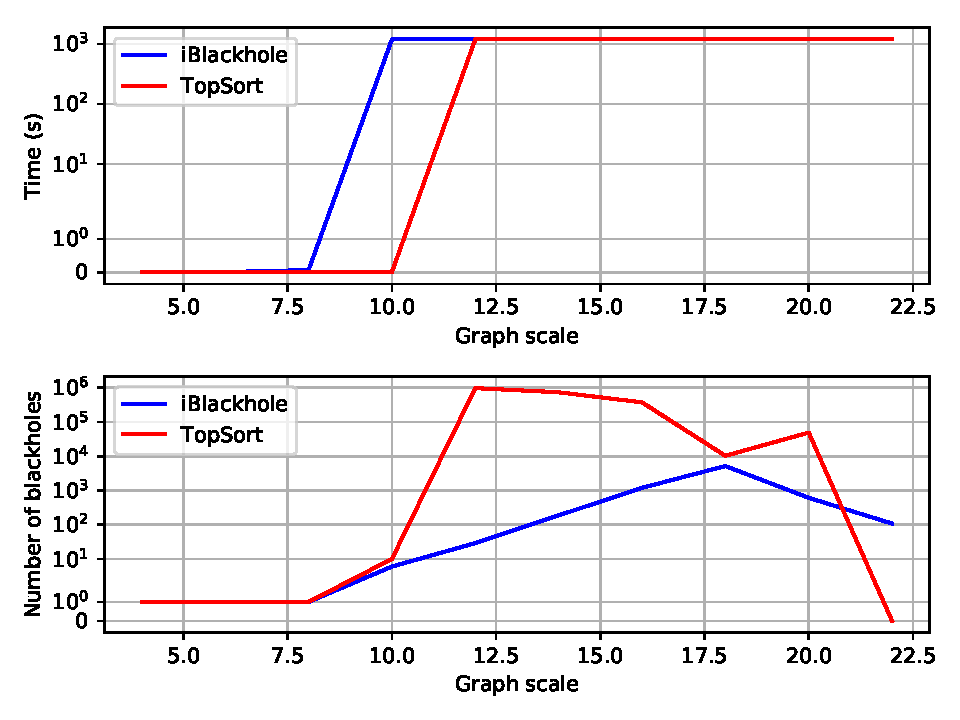
\includegraphics[width=\linewidth]{rmat.pdf}
	\caption{Algorithm results on RMAT graphs.}
	\label{fig:rmat}
\end{figure}

As it is shown in the Figures \ref{fig:rmat}, \ref{fig:ssca2} and \ref{fig:ur}, our TopSort approach to blackhole search shows better performance on small RMAT graphs and it stays in advantage up to RMAT-22. Apparently, condensation preprocessing takes more time on larger graphs and increases time spent before finding
the first blackhole. Nevertheless, our algorithm shows significantly better performance in those cases when preprocessing saves more time. Also, we suppose
that total working time on large graphs for our algorithm will be less, and this is the point for the future work.

\FIXME{Это, вообще говоря, странно}
SSCA2 graphs in our survey can be characterized with absolute absence of SCCs consisting of more than one node. Preprocessing here does not allow to obtain any
certain advantage, but only takes time. As we can see, on small graphs our approach beats the iBlackhole algorithm, but slows down on larger graphs.
We guess that the reason is less efficient order of search for our algorithm. One used in iBlackHole will faster print smaller blackholes, and later will try
to find larger ones, meanwhile our approach will check blackholes of all sizes.

\begin{figure}[H]
	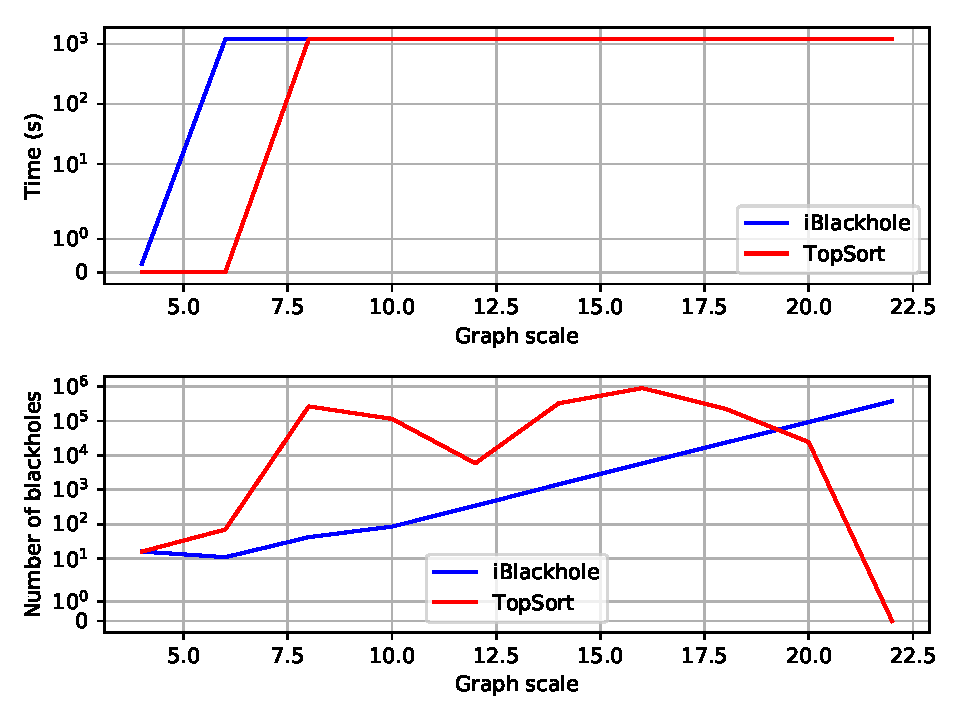
\includegraphics[width=\linewidth]{ssca2.pdf}
	\caption{Algorithm results on SSCA2 graphs.}
	\label{fig:ssca2}
\end{figure}
\begin{figure}[H]
	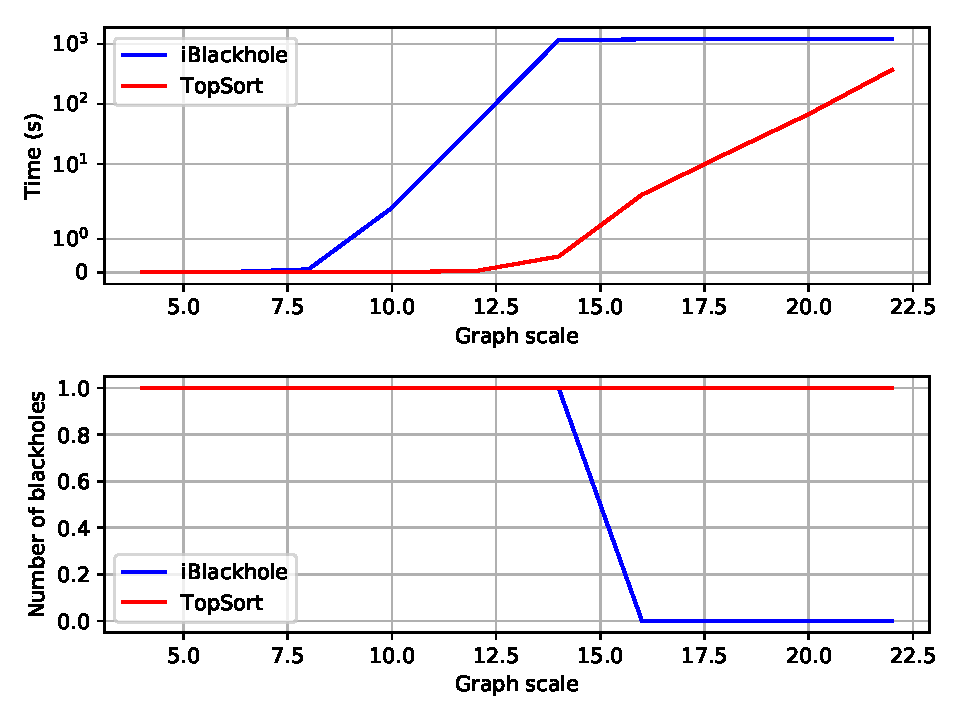
\includegraphics[width=\linewidth]{ur.pdf}
	\caption{Algorithm results on Uniform Random graph.}
	\label{fig:ur}
\end{figure}

Finally, we should point out, that our preprocessing dramatically speeds up blackhole search on the graphs, where no blackholes present at all. Brute force is
avoided completely in this case, making calculation time impressively small in comparison to the iBlackhole algorithm.


\section{Conclusion}

In this paper we addressed some issues in application of the already known iBlackhole algorithm. We introduced and tested two different ideas of optimization, combined into
our TopSort algorithm. Those are graph condensation preprocessing and topological sort of the brute-force optimization. We tested our approach on three different types of graphs and number of scales.

In case of graph with large strong connected components we demostrate definite advantage over the iBlackhole algorithm. Then, we can relatively fast in the case of total blackhole absence, but sometimes quite costly preprocessing
deminishes any performance boost and our advantage  degrades.
\FIXME{можно написать в TODO}
If we check blackhole sizes consecutively, what is the expected time of the first blackhole found? 

\textit{Comment for the reviewer}. In the final paper revision we enhance our TopSort algorithm, add its parallel implementation and present much detailed evaluation on the larger graphs. 

%
% ---- Bibliography ----
%
\bibliographystyle{spmpsci}
\bibliography{biblio}


\end{document}
